\documentclass[12pt,a4paper]{article}
\usepackage{amsmath,amscd,amsbsy,amssymb,latexsym,url,bm,amsthm}
\usepackage{epsfig,graphicx,subfigure}
\usepackage{enumitem,balance}
\usepackage{wrapfig}
\usepackage{mathrsfs, euscript}
\usepackage[usenames]{xcolor}
\usepackage{hyperref}
\usepackage[vlined,ruled,commentsnumbered,linesnumbered]{algorithm2e}
\usepackage{float}
\usepackage{array}
\usepackage{diagbox}
\usepackage{color}
\usepackage{indentfirst}
\usepackage{fancyhdr}
\usepackage{gensymb}
\usepackage{geometry}
\usepackage{setspace}
\usepackage{aurical}
\usepackage{times}
\usepackage{caption}
\usepackage{fontspec}
\usepackage{booktabs}
\setmainfont{Times New Roman}

\newtheorem{theorem}{Theorem}[section]
\newtheorem{lemma}[theorem]{Lemma}
\newtheorem{proposition}[theorem]{Proposition}
\newtheorem{corollary}[theorem]{Corollary}
\newtheorem{exercise}{Exercise}[section]
\newtheorem*{solution}{Solution}
\theoremstyle{definition}

\newcommand{\postscript}[2]
 {\setlength{\epsfxsize}{#2\hsize}
  \centerline{\epsfbox{#1}}}
\renewcommand{\baselinestretch}{1.0}

\setlength{\oddsidemargin}{-0.365in}
\setlength{\evensidemargin}{-0.365in}
\setlength{\topmargin}{-0.3in}
\setlength{\headheight}{0in}
\setlength{\headsep}{0in}
\setlength{\textheight}{10.1in}
\setlength{\textwidth}{7in}
\makeatletter \renewenvironment{proof}[1][Proof] {\par\pushQED{\qed}\normalfont\topsep6\p@\@plus6\p@\relax\trivlist\item[\hskip\labelsep\bfseries#1\@addpunct{.}]\ignorespaces}{\popQED\endtrivlist\@endpefalse} \makeatother
\makeatletter
\renewenvironment{solution}[1][Solution] {\par\pushQED{\qed}\normalfont\topsep6\p@\@plus6\p@\relax\trivlist\item[\hskip\labelsep\bfseries#1\@addpunct{.}]\ignorespaces}{\popQED\endtrivlist\@endpefalse} \makeatother

\begin{document}
\noindent
%==========================================================
\noindent\framebox[\linewidth]{\shortstack[c]{
\Large{\textbf{Report on Homework 3 -- SVM vs. Neural Networks}}\vspace{1mm}\\ 
CS420, Machine Learning, Shikui Tu, Summer 2018 \vspace{1mm} \\
Zelin Ye 515030910468}}

\section{Introduction}

In machine learning, SVM (Support Vector Machine) is a commonly used classfication method due to its high efficiency and accuracy. Recent years, the neural network has been attracting more and more attention, and also used to solve classification problems. In this homework, I would investigate the performances of SVM and neural network (e.g. MLP) on some classification datasets under different experimental settings (e.g. pass).

\section{Methodology}

In this section, I would introduce the datasets and models in my experiments.

\subsection{Datasets}

In my experiments, I use two datasets that are from \textbf{LIBSVM Data} \cite{dataA} to investigate the performances of SVM and neural network. One is \textbf{splice}, a binary classification dataset with 60 features, 1000 training samples and 2175 testing samples. Another is called \textbf{satimage}, which is for multi-class classification and has 36 features, 6 classes, 3104 training samples and 2000 testing samples.

Additionally, I choose a dataset called \textbf{ConvexNonConvex} from LISA \cite{dataB} to conduct comparison between SVM and deep learning algorithm benchmarks. It is a binary classification dataset that contains 784 features, 8000 training samples and 50000 testing samples.

More details about these datasets can refer to Appendix \ref{apd:dataset}.

\subsection{Models}

For neural network, considering the complexity of features and scale of samples, I choose MLP (Multi-layer Perceptron) instead of popular DNN or CNN.

\vspace{0.01\linewidth}
In experiments, I would investigate the performances of MLP under different architectures or parameter settings (e.g. number of hidden layers or hidden neurons).

\section{Experiments and Results}

\subsection{Preprocess}

Most datasets are likely to have missing data, and those in LIBSVM Data are no exception. Therefore, I first make up for the omission in the datasets, replacing empty data with corresponding mean values. Afterwards, I convert the labels from numbers to one-hot vectors for the calculation of loss.

\section{SVM}
\label{sec:svm}

In this section, I would show the performances of SVM in both \textit{splice} and \textit{satimage} datasets under different configurations (e.g. pass). Note that the two datasets have different problem settings, sample sizes and etc. I would thus conduct some pertinent discussion based on each experiment result.

\subsection{Binary Classification}

\subsection{Multi-class Classification}

\section{Neural Network}

In this section, I would also show the performances of MLP in the two datasets under different configurations (e.g. optimization algorithms, network architectures). Similarly, I would analyze each result like Sec. \ref{sec:svm}.

\subsection{Optimization Algorithm}

\begin{figure}[H]
	\centering
	\subfigure[Splice-Training Set]{
		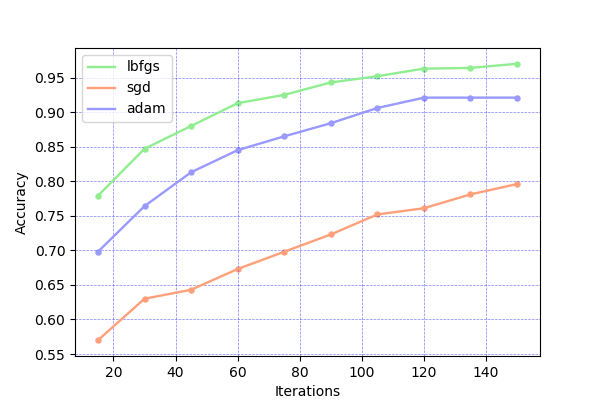
\includegraphics[width=0.45\linewidth]{img/mlp_optimizer_splice_tr.png}
	}
	\subfigure[Splice-Tetsing Set]{
		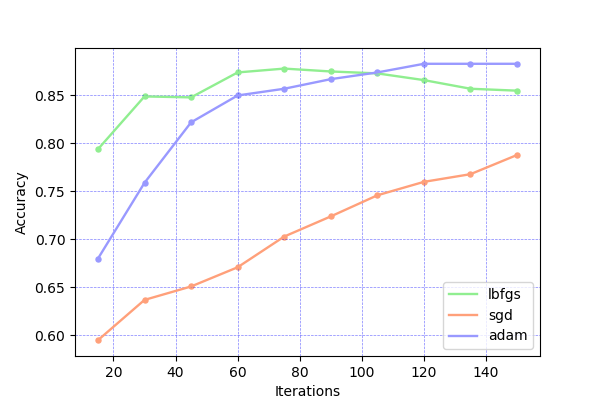
\includegraphics[width=0.45\linewidth]{img/mlp_optimizer_splice_t.png}
	}
	\subfigure[Satimage-Training Set]{
		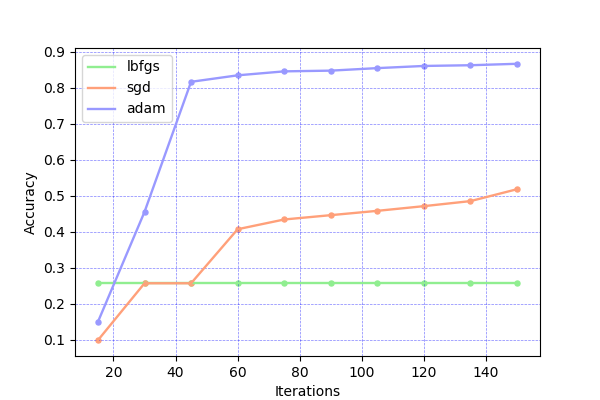
\includegraphics[width=0.45\linewidth]{img/mlp_optimizer_sat_tr.png}
	}
	\subfigure[Satimage-Testing Set]{
		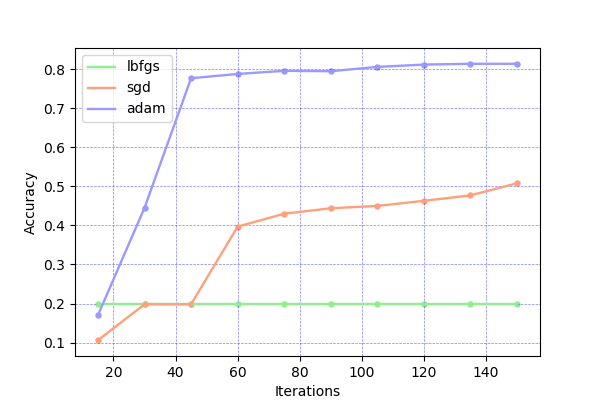
\includegraphics[width=0.45\linewidth]{img/mlp_optimizer_sat_t.png}
	}
	\caption{The performances of MLP under different optimization algorithms.}
	\label{fig:mlp-optimizer}
\end{figure}

\subsection{Activation Function}

\begin{figure}[H]
	\centering
	\subfigure[Splice-Training Set]{
		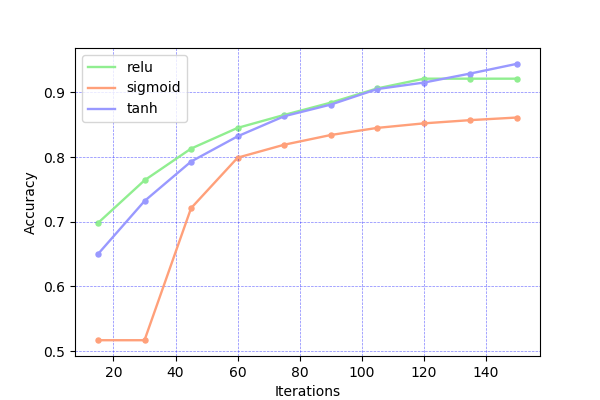
\includegraphics[width=0.45\linewidth]{img/mlp_activation_splice_tr.png}
	}
	\subfigure[Splice-Tetsing Set]{
		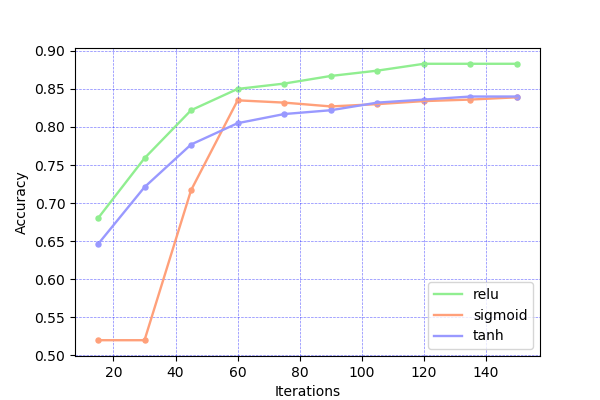
\includegraphics[width=0.45\linewidth]{img/mlp_activation_splice_t.png}
	}
	\subfigure[Satimage-Training Set]{
		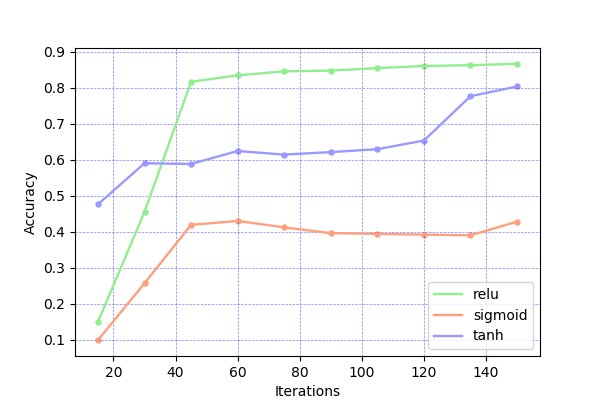
\includegraphics[width=0.45\linewidth]{img/mlp_activation_sat_tr.png}
	}
	\subfigure[Satimage-Testing Set]{
		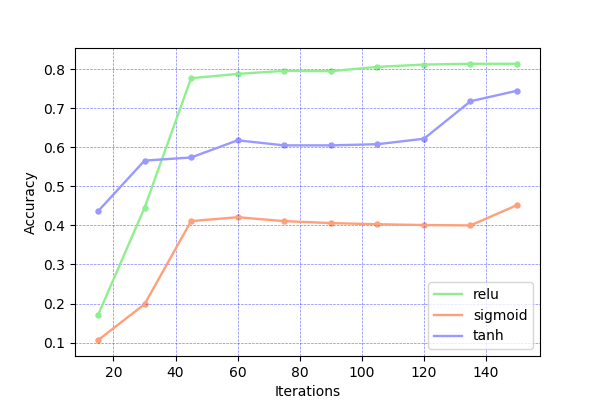
\includegraphics[width=0.45\linewidth]{img/mlp_activation_sat_t.png}
	}
	\caption{The performances of MLP under different activation functions.}
	\label{fig:mlp-activation}
\end{figure}

\subsection{Learning Rate}

\begin{figure}[H]
	\centering
	\subfigure[Splice]{
		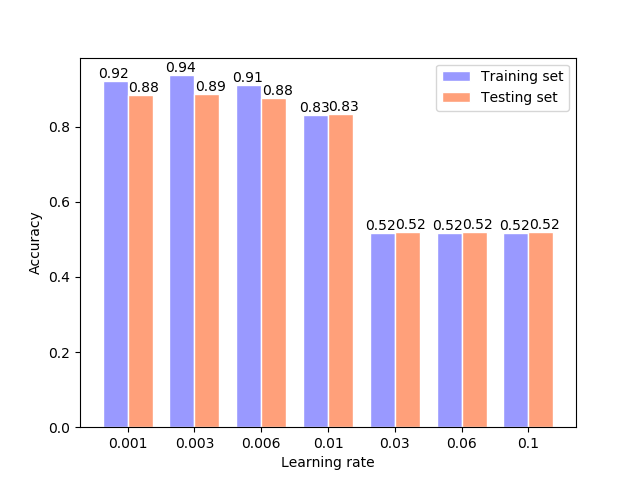
\includegraphics[width=0.45\linewidth]{img/mlp_lr_splice.png}
	}
	\subfigure[Satimage]{
		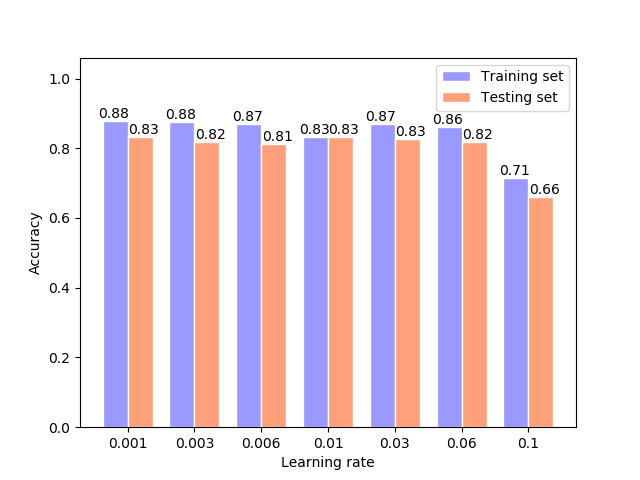
\includegraphics[width=0.45\linewidth]{img/mlp_lr_sat.png}
	}
	\caption{The performances of MLP under different learning rate.}
	\label{fig:mlp-lr}
\end{figure}

\subsection{Network Architecture}

\subsection{Dimension of Features}

\begin{figure}[H]
	\centering
	\subfigure[Splice-Training Set]{
		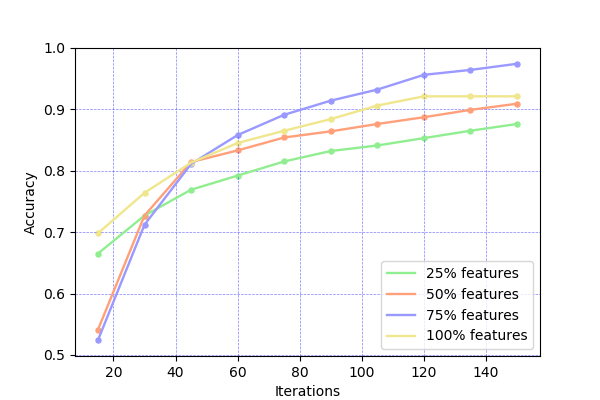
\includegraphics[width=0.45\linewidth]{img/mlp_dim_splice_tr.png}
	}
	\subfigure[Splice-Tetsing Set]{
		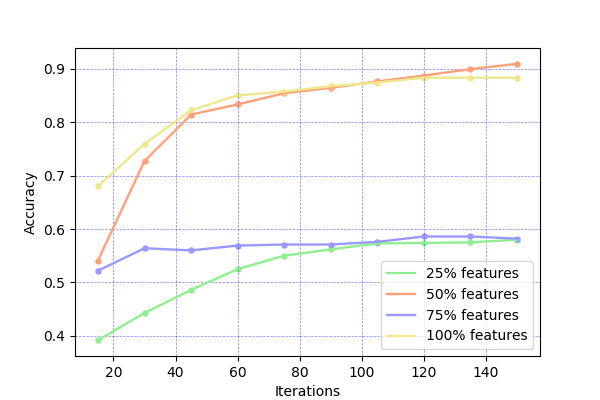
\includegraphics[width=0.45\linewidth]{img/mlp_dim_splice_t.png}
	}
	\subfigure[Satimage-Training Set]{
		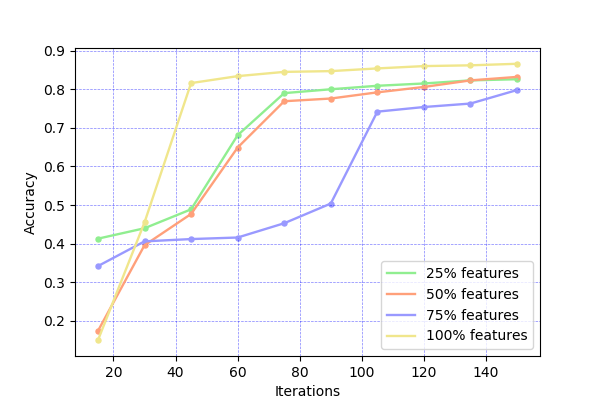
\includegraphics[width=0.45\linewidth]{img/mlp_dim_sat_tr.png}
	}
	\subfigure[Satimage-Testing Set]{
		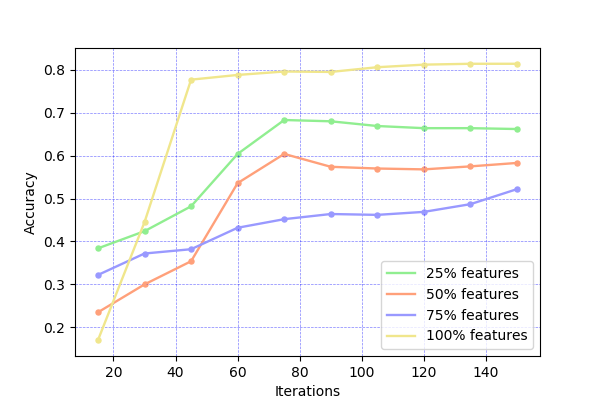
\includegraphics[width=0.45\linewidth]{img/mlp_dim_sat_t.png}
	}
	\caption{The performances of MLP under different dimensions of features.}
	\label{fig:mlp-dim}
\end{figure}

\section{Comparison Between SVM and Deep Learning Algorithm Benchmark}

\newpage
\begin{appendix}
\section{Appendix}

\subsection{Details of Datasets in Experiments}
\label{apd:dataset}

\subsubsection{Splice \cite{splice}}

Basically, according to the biological knowledge, splice junctions are points on a DNA sequence at which `superfluous' DNA is removed during the process of protein creation in higher organisms.

\vspace{0.01\linewidth}
Splice dataset aims to recognize two classes of splice junctions, given a DNA sequence, the boundaries between exons (the parts of the DNA sequence retained after splicing) and introns (the parts of the DNA sequence that are spliced out).

\subsubsection{Satimage \cite{satimage}}

Satimage dataset is also called \textbf{satalog} dataset. It contains multi-spectral values of pixels in 3 $\times$ 3 neighbourhoods in satellite images, and the classification associated with the central pixel in each neighbourhood.

\vspace{0.01\linewidth}
As a classification dataset, the aim of satimage is to predict the classification, given the multi-spectral values. In the sample database, the class of a pixel is coded as a number.

\subsubsection{ConvexNonConvex \cite{convex}}

The ConvexNonConvex dataset consists of convex regions with pixels of value 255. Such regions are constructed via the intersection of a number of half-planes whose location and orientation were chosen uniformly at random. In the meanwhile, the number of half-planes is also sampled randomly according to a geometric distribution with parameter 0.195.

\vspace{0.01\linewidth}
To ensure the validity of the data, a candidate convex image is rejected once there are less than 19 pixels in it.


\end{appendix}

\bibliographystyle{ieeetr}
\bibliography{bio}

\end{document}